\documentclass{article}
\usepackage[T1]{fontenc}

\usepackage{graphicx}
\usepackage{listings}
\begin{document}

\title{FOSS Lab Report}
\author{Gokul K\\[2\baselineskip]
Roll Number: 21\\[2\baselineskip]}
\date{25 January 2020}

\maketitle

\setcounter{section}{4}
\section{Shell Programming II}
\subsection{Aim}
Write shell script to show various system configurations like\newline
  1) your OS and version, release number, kernel version\newline
  2) all available shells\newline
  3) computer CPU information like processor type, speed etc\newline
  4) memory information\newline
  5) hard disk information like size of hard-disk, cache memory, model etc\newline
  6) File system (Mounted)\newline
\subsection{Source Code}
\begin{verbatim}
#! /bin/bash
echo -e "`cat /etc/os-release`"
echo -e "`cat /etc/shells/`"
echo -e "`xset q`"
echo -e "`cat /proc/meminfo`"
echo -e "Driver: `sudo hdparm -I /dev/sda`"
echo -e "`cat /proc/mounts`"
\end{verbatim}

\subsection{Output}
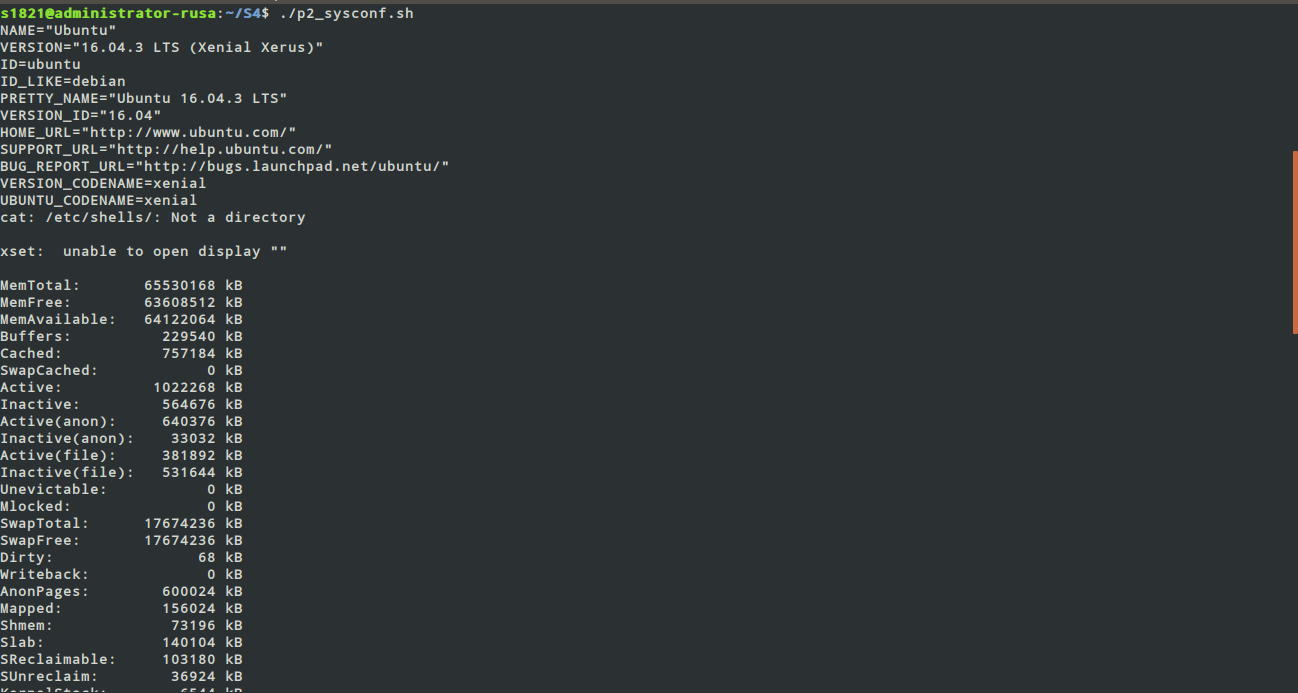
\includegraphics[width=0.9\textwidth]{img/p5/ss1.png}\newline
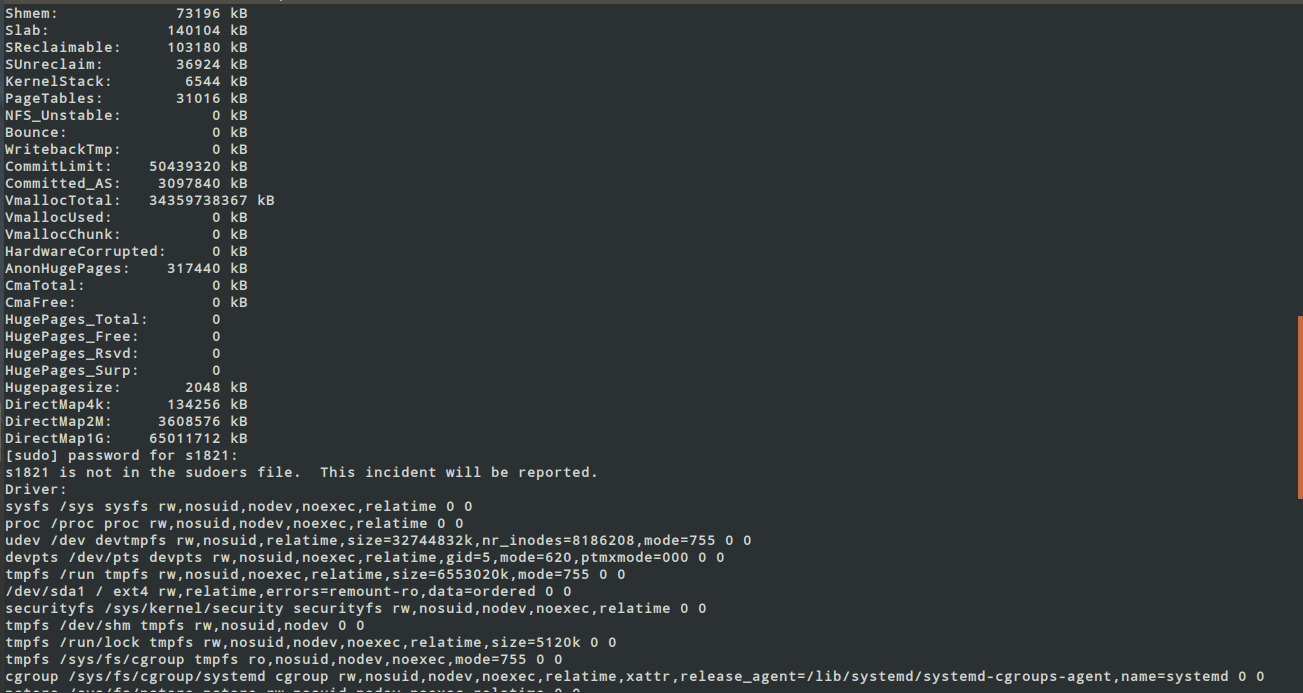
\includegraphics[width=0.9\textwidth]{img/p5/ss2.png}\newline
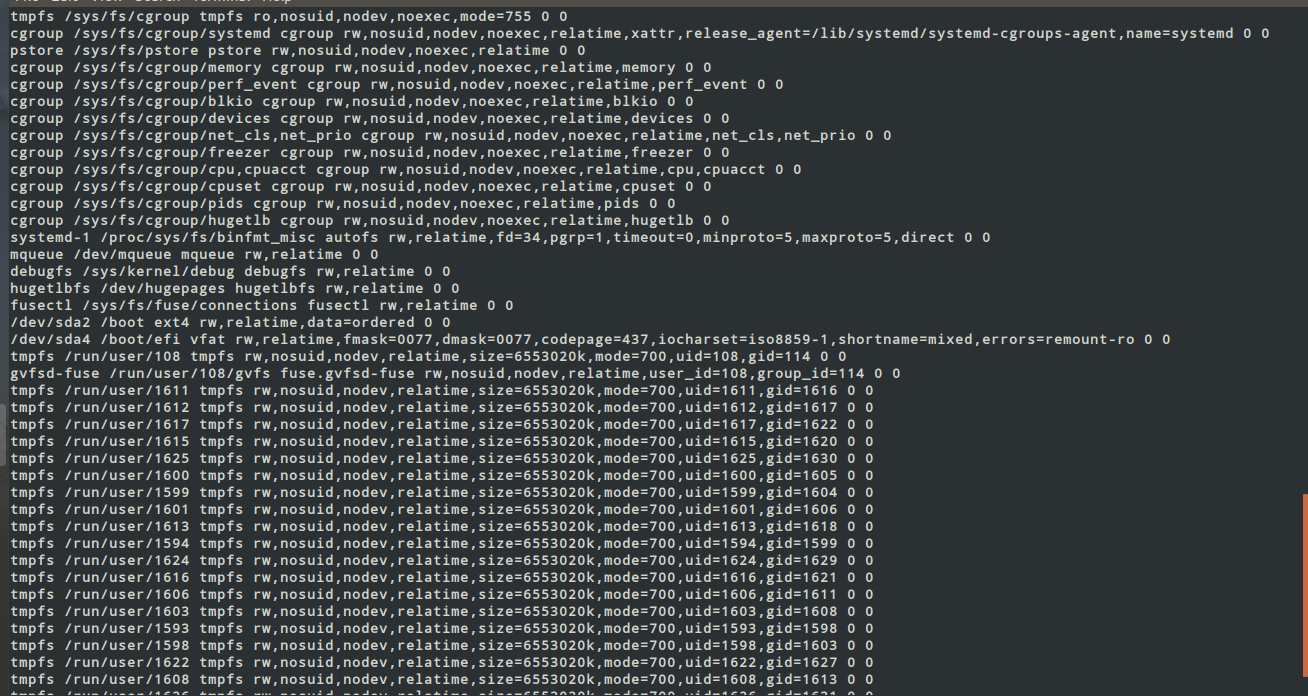
\includegraphics[width=0.9\textwidth]{img/p5/ss3.png}

\subsection{Result}
The above program is run on the server shell and the output is recorded. Since administrator privilege is not given, the driver details could not be printed. 
\end{document}